\documentclass[tikz]{standalone}
\usepackage{pgfplots}
\pgfplotsset{compat=1.18}
\definecolor{utnblue}{RGB}{0, 102, 204}

\begin{document}
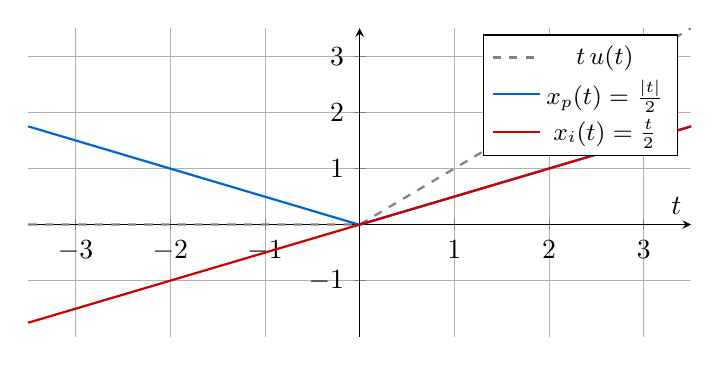
\begin{tikzpicture}
    \begin{axis}[
        width=10cm, height=5.5cm,
        axis lines=middle,
        xmin=-3.5, xmax=3.5, ymin=-2, ymax=3.5,
        xlabel={$t$}, ylabel={},
        grid=both,
        grid style={line width=.1pt, draw=gray!40},
        major grid style={line width=.2pt, draw=gray!60},
        xtick={-3,-2,-1,0,1,2,3},
        ytick={-1,0,1,2,3},
        legend style={at={(0.98,0.98)}, anchor=north east, font=\small},
        every axis plot/.append style={thick},
    ]
    % Señal original r(t) = t u(t)
    \addplot[gray, dashed] coordinates {(-3.5,0) (0,0) (3.5,3.5)};
    \addlegendentry{$t\,u(t)$}
    % Componente par = |t|/2
    \addplot[utnblue] coordinates {(-3.5,1.75) (-0.01,0) (0.01,0) (3.5,1.75)};
    \addlegendentry{$x_p(t) = \frac{|t|}{2}$}
    % Componente impar = t/2
    \addplot[red!80!black] coordinates {(-3.5,-1.75) (3.5,1.75)};
    \addlegendentry{$x_i(t) = \frac{t}{2}$}
    \end{axis}
\end{tikzpicture}
\end{document}
